The main dogma of biology states: information in a cell flows from DNA to RNA and then to proteins. Although the actual working of the cell is much more comlpex to be
contained in any dogma, it captures a large picture of the state-of-art of our understanding of the working of a cell. Proteins in this picture have a crucial place:
they are the cogs of the cell machinery. These are the protein expressed in a cell and their interactions that mainly define phenotype of that cell. Therefore gainig new 
data on the protein interaction in a cell profoundly enhances our capabilities to understand and change living organisms for the needs of the society.

\subsection{Classification of protein-protein interactions}
Commonly used classification of the protein-protein complexes uses the following main criteria: composition of a complex, its lifetime and stability \cite{nooren2003diversity}.

\subsubsection{Protein composition and interface}
The complex can be comprised of two identical or highly homologous proteins. An example of such a complex is the D-alanyl carrier protein (pdb code 4BPG), which consists of two identical
polypeptide chains (Fig. \ref{fig:exampleHomoDimer}). The proteins of this class are called homo-oligomers. On the other hand, if the complex consists of two distinct proteins it is named hetero-oligomer. 
An example of hetero-dimer (Glycosidase CelD bound to artificial affitin E12 protein, \cite{correa2014potent}, pdb code 4CJ0) is shown on Fig \ref{fig:exampleHeteroDimer}. 
Homo-oligomers are further divided dependent on the interface of oligomerization. If the two chains bind using the identical binding interace, their complex is called isologous. 
We can see that D-alanyl carrier protein is an example of isologous homodimer (Fig. \ref{fig:exampleHeteroDimer}). On the contrary, the homo-oligomeric assemblies where proteins bind through distinct
interfaces are called heterologous. 
%An example of the protein of this class is the abalone egg lysin dimer (pdb code 1LYN, \cite{shaw1995crystal}, Fig \ref{}). 
\begin{figure}[!ht]
\label{Fig:Step1Purification}
    \begin{minipage}{0.49\linewidth}
    \begin{centering}
      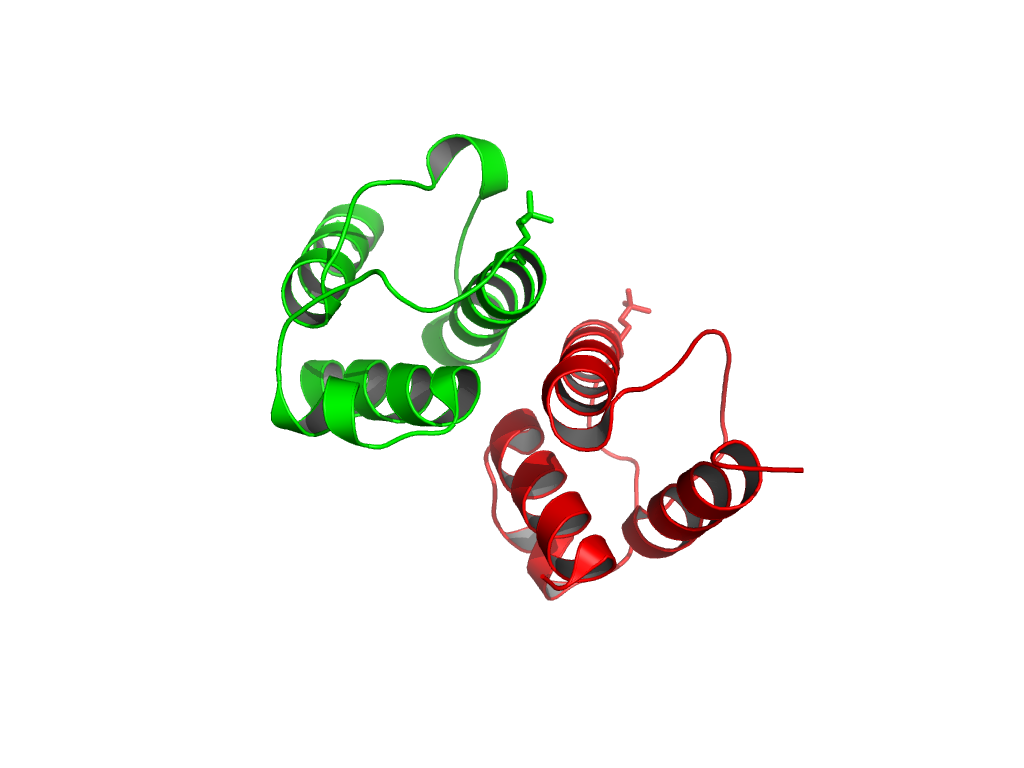
\includegraphics[width=1\linewidth]{Intro/Fig/HomoDimer.png}  
      \caption[Example of a homodimeric complex]{Example of a homodimeric complex,  D-alanyl carrier protein, pdb code 4BPG.}\label{fig:exampleHomoDimer}
    \end{centering}
    \end{minipage}
    \hfill
    \begin{minipage}{0.49\linewidth}
    \begin{centering}
      \includegraphics[width=1\linewidth]{Intro/Fig/HeteroDimer.png}  
      \caption[Example of a heterodimeric complex]{Example of a heterodimeric complex,  Glycosidase CelD bound to artificial affitin E12 protein, \cite{correa2014potent}, pdb code 4CJ0}\label{fig:exampleHeteroDimer}
    \end{centering}
    \end{minipage}
\end{figure}


\subsubsection{Stability of protomers}
The proteins that form a complex can be either stable or not on their own \emph{in vivo}. In the first case, when a complex is formed out of stable proteins it is called \emph{non-obligate}.
In many cases these proteins are localized in different compartements of a cell. Usually, interactions between receptor-ligand, enzyme-inhibitor, \emph{etc} belong to
non-obligate interactions. In the other case when a complex of one or both chains do not exist as folded proteins on their own, it is called \emph{obligate}.
An example of such a complex is the Arc repressor dimer, which consists of two peptide chains. Upon dimerization (catalized by DNA \cite{marcovitz2009arc}) these chains 
obtain stable secondary structure, that was absent in the monomer.

\subsubsection{Complex lifetime}
If two proteins form a very stable complex they said to interact \emph{permanently}. In many cases obligate complexes, such as Arc repressor dimer, are permanent.
On the other hand, if a complex is dissociated and formed continuously \emph{in vivo}, the interaction between its constituting proteins is called \emph{transient}. 
Many of non-obligate interactions are also transient. However, there are strong transient interactions that require the presense of some molecule for the complex 
dissociation. An example of a strong transient interaction is the formation of trimeric G protein, for which guanine triphosphate is the dissociation trigger.